\section{数值实验}\label{sec:exp}

\subsection{实验设计}\label{sec:design}
表\ref{tab:policies}列出参与比较的策略。前五种是在线策略，\SeqDP{} 预知整条类型序列，只作为策略损失的基准。所有策略在全部实验中使用相同的规则与参数，没有针对任何数据集调整。

\begin{table}[htbp]
\centering\small
\caption{参与比较的策略}\label{tab:policies}
\begin{tabularx}{\linewidth}{@{}l X l l@{}}
\toprule
策略 & 推荐规则 & 决策所用信息 & 每期计算\\
\midrule
\AlgOne{} & 题目算法 1：按 $v_{ij}$ 固定推荐前 $K$ 件，不检查库存 & $i_t$ & 无\\
\Greedy{} & 在有货商品中按 $v_{ij}$ 推荐前 $K$ 件 & $i_t,\ c_t$ & 排序\\
\LPDual{} & 算法\ref{alg:dual}，机会成本取对偶价格\eqref{eq:theta_dual} & $i_t,\ c_t,\ \tau,\ \lambda$ & 1 个 LP\\
\LPFD{} & 算法\ref{alg:dual}，机会成本取有限差分\eqref{eq:theta_fd} & $i_t,\ c_t,\ \tau,\ \lambda$ & $\le n+1$ 个 LP\\
\LPCount{} & \LPDual{}，需求预测改用剩余人数\eqref{eq:countforecast} & $i_t,\ c_t,\ n_t,\ N$ & 1 个 LP\\
\IIDDP{} & 式\eqref{eq:iiddp}的最优动作表 & $i_t,\ c_t,\ \tau,\ \lambda$ & 查表\\
\SeqDP{} & 式\eqref{eq:seqdp}的最优动作，预知 $i_{1:T}$ & $i_{1:T},\ c_t$ & 基准\\
\bottomrule
\end{tabularx}
\end{table}

实验分为六组：
\begin{enumerate}[label=(\arabic*)]
\item 题目给出的五份数据：精确评价各策略，并对每份数据做 $B=2000$ 次蒙特卡洛重复（第\ref{sec:main}--\ref{sec:where}节）；
\item 1000 条生成序列：500 条人数为 $(50,30,20)$ 的随机排列，500 条按 $\lambda$ 独立同分布生成的序列（第\ref{sec:random}节）；
\item 六种分块到达顺序，检验需求预测失准时的表现（第\ref{sec:order}节）；
\item 库存缩放 $\theta\in\{0.3,0.4,\ldots,1.2\}$ 与推荐位数 $K\in\{1,2,3\}$（第\ref{sec:sens}节）；
\item 销售期 $T$ 从 25 增至 1600、库存同比例放大（第\ref{sec:scale}节）；
\item 随机生成的较大实例，最大为 $(m,n,T,K)=(20,30,300,4)$（第\ref{sec:scale}节）。
\end{enumerate}
第 (1)--(4) 组的期望值均由第\ref{sec:exact}节的方法精确计算，第 (5)、(6) 组的状态空间过大，采用蒙特卡洛模拟。计算环境为 Python 3.11.9、Gurobi 13.0.3（单线程对偶单纯形法）、NumPy 1.26.4。

\subsection{五份数据上的结果}\label{sec:main}
表\ref{tab:main}给出主策略 \LPDual{} 的逐份结果，表\ref{tab:aggregate}汇总各策略的表现。\LPDual{} 在五份数据上的平均期望收入为 \ERDual{}，达到离线上界 706 的 \RatioDual\%；平均遗憾 $\overline G=\GavgDual$，最大遗憾 $G_{\max}=\GmaxDual$，全部推荐满足库存约束。期末平均剩余商品 1 \EconeDual{} 件、商品 2 \EctwoDual{} 件、商品 3 \EcthreeDual{} 件，商品 1 在 \SoldOutEndDual\% 的路径上售罄。商品 2、3 的剩余量与流体解的剩余量 $\bar c=(0,\,6,\,38/3)$ 接近，说明商品 2、3 本身库存充裕，剩余是需求不足的自然结果；商品 1 是唯一的稀缺商品。

\begin{table}[htbp]
\centering\small
\caption{\LPDual{} 在五份数据上的期望结果与首次模拟}\label{tab:main}
\begin{tabular}{lrrrrrr}
\toprule
指标 & D1 & D2 & D3 & D4 & D5 & 五组均值 \\
\midrule
\multicolumn{7}{l}{\textit{固定到达序列，对购买结果取期望}} \\
期望收入 $\E R_T$ & 695.854 & 696.397 & 695.260 & 696.130 & 695.827 & 695.894 \\
期望遗憾 $G_s$ & 10.146 & 9.603 & 10.740 & 9.870 & 10.173 & 10.106 \\
策略损失 $L_s$ & 0.099 & 0.090 & 0.215 & 0.225 & 0.214 & 0.169 \\
商品 1 期末库存 & 0.907 & 0.894 & 0.905 & 0.897 & 0.912 & 0.903 \\
商品 2 期末库存 & 6.177 & 6.183 & 6.175 & 6.179 & 6.175 & 6.178 \\
商品 3 期末库存 & 12.610 & 12.533 & 12.716 & 12.579 & 12.608 & 12.609 \\
商品 1 售罄概率 & 70.8\% & 71.9\% & 71.6\% & 71.8\% & 71.7\% & 71.6\% \\
\midrule
模拟均值 $\overline R_s$ & 696.237 & 697.303 & 695.309 & 695.564 & 695.891 & 696.061 \\
95\% 区间半宽 $h_s$ & 1.250 & 1.230 & 1.234 & 1.216 & 1.248 & -- \\
\midrule
\multicolumn{7}{l}{\textit{每份数据的首次购买模拟}} \\
实现收入 $R_T^{(1)}$ & 678 & 710 & 680 & 660 & 656 & 676.8 \\
实现遗憾 $F_s-R_T^{(1)}$ & 28 & -4 & 26 & 46 & 50 & 29.2 \\
期末库存 & $(0,10,12)$ & $(0,3,16)$ & $(5,2,14)$ & $(0,13,11)$ & $(0,12,13)$ & -- \\
\bottomrule
\end{tabular}
\par\vspace{0.35em}{\footnotesize 五份数据的 $F_s$ 均为 706。期望值和售罄概率由精确递推得到。每份数据的首次模拟均使用预设随机流的首组购买抽样，五条路径共出现 \FirstOosSlots{} 次缺货推荐。期望遗憾的最大值为 \GmaxDual，首次模拟的最大实现遗憾为 \FirstMaxRegret。}
\end{table}

\begin{table}[htbp]
\centering\small
\caption{各策略在五份数据上的综合表现}\label{tab:aggregate}
\begin{tabular}{lrrrrrr}
\toprule
策略 & $\overline{\E R_T}$ & $\overline G$ & $G_{\max}$ & $\overline G^{\,\mathrm{MC}}$ & $\overline L$ & $\overline W$ \\
\midrule
\AlgOne{} & 693.394 & 12.606 & 12.606 & 12.426 & 2.669 & 6.29 \\
\Greedy{} & 695.550 & 10.450 & 11.168 & 10.318 & 0.513 & 0.00 \\
\LPFD{} & 695.490 & 10.510 & 11.058 & 10.306 & 0.572 & 0.00 \\
\LPDual{} & 695.894 & 10.106 & 10.740 & 9.939 & 0.169 & 0.00 \\
\LPCount{} & 695.768 & 10.232 & 11.147 & 10.121 & 0.295 & 0.00 \\
\IIDDP{} & 695.862 & 10.138 & 10.815 & 9.995 & 0.201 & 0.00 \\
\SeqDP{} & 696.062 & 9.938 & 10.525 & -- & 0.000 & -- \\
\bottomrule
\end{tabular}
\par\vspace{0.35em}{\footnotesize $\overline G$ 与 $G_{\max}$ 按式\eqref{eq:avgmax}由精确期望计算；$\overline G^{\,\mathrm{MC}}=\frac15\sum_s(F_s-\overline R_s)$ 为模拟估计；$\overline L$ 为五份数据上策略损失 $L_s$ 的平均；$\overline W$ 为每条路径上缺货推荐的期望次数，定义见式\eqref{eq:waste}。\LPCount{} 使用了总人数 $N$；\SeqDP{} 预知顾客类型序列，只作为基准。}
\end{table}


与其他策略相比：
\begin{itemize}
\item \LPDual{} 在全部五份数据上都高于 \Greedy{}，期望收入差为 \DualGreedyMin--\DualGreedyMax；在 \DualFDWins{} 份数据上高于 \LPFD{}，平均高 \DualFDAvg。
\item \IIDDP{} 是独立同分布到达假设下的最优在线策略，在五份数据上的平均期望收入为 \ERIID{}。它在 4 份数据上高于 \LPDual{}（差距不超过 0.22），但在数据 1 上低 0.67，平均因而略低于 \LPDual{}。\IIDDP{} 为后段可能到来的类型 2 顾客保留安全库存（预留阈值约为 \LPDual{} 的两倍，见图\ref{fig:threshold}）。数据 1 的第 91--93 期连续到达 3 位类型 1 顾客，\IIDDP{} 不向他们推荐商品 1，而第 94--100 期只有 3 位类型 2 顾客，保留的商品 1 有一部分没能售出：它在数据 1 上的策略损失有 99\% 属于多留，集中在第 92、93 期，期末商品 1 的售罄概率只有 58\%，\SeqDP{} 为 72\%。第\ref{sec:random}节的 1000 条生成序列上，\IIDDP{} 平均更优，五份数据上的平均排序受数据 1 影响。
\item \SeqDP{} 的平均期望收入为 \ERSeq，是任何在线策略在这五份数据上的上限。\LPDual{} 的平均策略损失为 \LavgDual，即使预知全部顾客类型，期望收入也只能再提高这么多。
\item 算法 1 在五份数据上的期望收入都是 \AlgOneER{}，平均每条路径出现 \AlgOneOOS{} 次缺货推荐，比 \Greedy{} 低 \AlgOneLossGreedy。
\end{itemize}

模拟结果与精确值吻合：五种可模拟策略在五份数据上的 \MCtotal{} 个模拟均值中，有 \MCinside{} 个落在精确值的 95\% 置信区间内，标准化偏差 $|\overline R_s-\E R_T|\sqrt B/\hat\sigma_s$ 的最大值为 \MCmaxZ。需要注意，$B=2000$ 时单个策略的置信区间半宽约为 \MChw，大于策略之间 0.3--0.9 的期望收入差异，仅凭模拟均值无法可靠地给策略排序。公共随机数大幅降低了配对比较的方差：\LPDual{} 与 \Greedy{} 在 \MCpairEqual\% 的重复中收入完全相同，配对差的半宽只有约 \MCpairhw。精确评价彻底消除了这一不确定性。图\ref{fig:mainloss}按数据集给出四种策略的策略损失。

\begin{figure}[htbp]
\centering
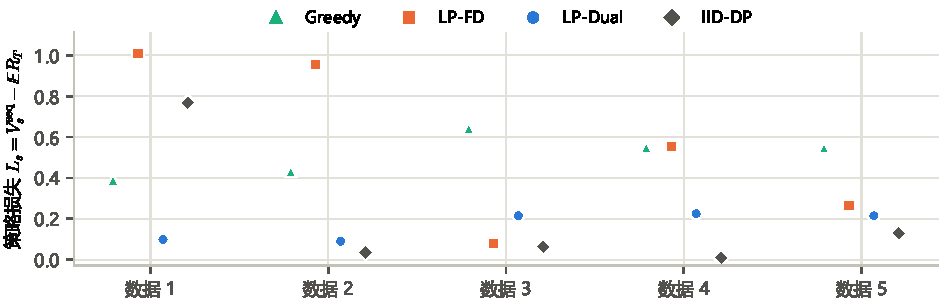
\includegraphics[width=\linewidth]{figures/main_loss.pdf}
\caption{五份数据上各策略的策略损失 $L_s=V^{\seq}_s-\E R_T$（精确值）}
\label{fig:mainloss}
\end{figure}

\subsection{遗憾的构成}\label{sec:decomp}
按式\eqref{eq:gap}分解，五份数据的流体松弛间隙 $F_s-V^{\seq}_s$ 介于 \FluidGapMin{} 与 \FluidGapMax{} 之间，平均为 \FluidGap，占 \LPDual{} 平均遗憾的 \FluidShare\%。换言之，\LPDual{} 的遗憾几乎全部来自流体模型与随机系统之间的差异，在线决策本身造成的损失只有 \LavgDual。

由于 $R_T=\sum_jr_j(C_j-c_{T+1,j})$ 且 $F=\sum_jr_js^{*}_j$（$s^{*}=(40,29,37/3)$ 为流体最优销量），期望遗憾可以按商品精确分解：
\begin{equation}
G_s=\sum_{j=1}^{n}\delta_j,\qquad \delta_j=r_j\bigl(\E c_{T+1,j}-\bar c_j\bigr),\qquad \bar c_j=C_j-s^{*}_j,
\label{eq:productgap}
\end{equation}
其中 $\bar c=(0,\,6,\,38/3)$ 是流体解的剩余库存，$\delta_j$ 是商品 $j$ 比流体解多剩下的库存所对应的收入。表\ref{tab:product}显示，\LPDual{} 的遗憾中有 \ContribOneDual（\ContribOneShare\%）来自商品 1 的剩余。流体解恰好卖完 40 件商品 1，随机系统做不到这一点。若每位类型 1、2 顾客都看到商品 1，商品 1 的潜在购买次数 $D_1=\mathrm{Bin}(50,0.6)+\mathrm{Bin}(30,0.4)$ 的均值为 42、标准差为 \DemandOneSd，$\Pr(D_1<40)=\DemandOneShort\%$，$\E(40-D_1)^+=\DemandOneLeft$。也就是说，即使从不预留商品 1，期末平均仍会剩下约 0.92 件，对应约 9.2 的收入。这部分剩余由需求的随机性决定，预知顾客类型的 \SeqDP{} 也剩下 \EconeSeq{} 件。

\begin{table}[htbp]
\centering\small
\caption{按商品分解的期望遗憾（五份数据平均），$\delta_j$ 的定义见式\eqref{eq:productgap}}\label{tab:product}
\begin{tabular}{lrrrrrrr}
\toprule
策略 & $\E c_{T+1,1}$ & $\E c_{T+1,2}$ & $\E c_{T+1,3}$ & $\delta_1$ & $\delta_2$ & $\delta_3$ & $\overline G=\sum_j\delta_j$ \\
\midrule
\AlgOne{} & 0.923 & 6.172 & 13.000 & 9.228 & 1.378 & 2.000 & 12.606 \\
\Greedy{} & 0.911 & 6.172 & 12.660 & 9.113 & 1.378 & -0.040 & 10.450 \\
\LPFD{} & 0.987 & 6.194 & 12.514 & 9.871 & 1.552 & -0.914 & 10.510 \\
\LPDual{} & 0.903 & 6.178 & 12.609 & 9.029 & 1.423 & -0.346 & 10.106 \\
\IIDDP{} & 0.935 & 6.185 & 12.552 & 9.351 & 1.476 & -0.688 & 10.138 \\
\SeqDP{} & 0.904 & 6.188 & 12.566 & 9.037 & 1.507 & -0.607 & 9.938 \\
\bottomrule
\end{tabular}
\end{table}


收入的随机波动远大于策略间的差异。图\ref{fig:dist}给出 \LPDual{} 在数据 1 上的精确收入分布：标准差约为 \SdDual，单条路径的收入超过 $F=706$ 的概率为 \ProbAboveFDOne\%（五份数据为 \PnegDualMin\%--\PnegDualMax\%），这些路径的样本遗憾为负。题目要求的遗憾若按单次实现计算，主要反映购买结果的运气。本文因此以条件期望 $\E[R_T\mid s]$ 定义 $G_s$，并在表\ref{tab:main}中同时报告模拟均值与置信区间。

\begin{figure}[htbp]
\centering
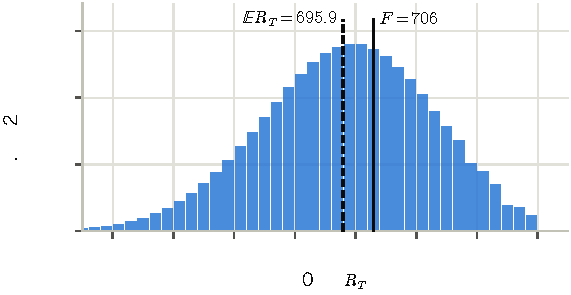
\includegraphics[width=0.66\linewidth]{figures/revenue_dist.pdf}
\caption{\LPDual{} 在数据 1 上的总收入 $R_T$ 的精确分布}
\label{fig:dist}
\end{figure}

\subsection{策略损失的来源}\label{sec:where}
为了定位策略损失，以 \SeqDP{} 的价值函数为尺度评价每一期的决策。令
\begin{equation}
Q_t(c,S)=\sum_{j\in S}p_{i_tj}\bigl[r_j+V_{t+1}(c-e_j)-V_{t+1}(c)\bigr],\qquad Q^{*}_t(c)=\max_{S\subseteq A(c),|S|\le K}Q_t(c,S),
\end{equation}
由 $V_t=V_{t+1}+Q^{*}_t$ 逐期展开，对任意策略 $\pi$ 有
\begin{equation}
L_s(\pi)=\sum_{t=1}^{T}\E_{\pi}\bigl[Q^{*}_t(c_t)-Q_t(c_t,S^{\pi}_t)\bigr],
\label{eq:pdl}
\end{equation}
求和中的每一项都非负，表示第 $t$ 期决策相对最优决策的期望损失，期望按策略 $\pi$ 自身的库存分布计算。本文用第\ref{sec:exact}节的前向递推精确计算式\eqref{eq:pdl}，数值上 $|\sum_t(\cdot)-L_s|\le\LossIdentityErr$。按决策类型，把每一期的损失分为三类：$L^{\mathrm{sell}}$ 为类型 1 顾客看到了最优决策不推荐的商品 1（多卖），$L^{\mathrm{hold}}$ 为类型 1 顾客没有看到最优决策推荐的商品 1（多留），$L^{\mathrm{oth}}$ 为其余决策的损失；再按时段把损失分为 $L_{[1,60]}$、$L_{[61,90]}$、$L_{[91,100]}$。

\begin{table}[htbp]
\centering\small
\caption{策略损失按决策类型与时段的分解（五份数据平均）}\label{tab:loss}
\begin{tabular}{lrrrrrrr}
\toprule
策略 & $\overline L$ & $\overline L^{\mathrm{sell}}$ & $\overline L^{\mathrm{hold}}$ & $\overline L^{\mathrm{oth}}$ & $\overline L_{[1,60]}$ & $\overline L_{[61,90]}$ & $\overline L_{[91,100]}$ \\
\midrule
\Greedy{} & 0.513 & 0.357 & 0.000 & 0.156 & 0.007 & 0.438 & 0.068 \\
\LPFD{} & 0.572 & 0.010 & 0.530 & 0.032 & 0.003 & 0.093 & 0.476 \\
\LPDual{} & 0.169 & 0.112 & 0.010 & 0.046 & 0.003 & 0.099 & 0.067 \\
\IIDDP{} & 0.201 & 0.020 & 0.155 & 0.025 & 0.000 & 0.045 & 0.155 \\
\bottomrule
\end{tabular}
\end{table}


表\ref{tab:loss}与图\ref{fig:losstime}给出三种策略各自的失误模式：
\begin{itemize}
\item \Greedy{} 的主要损失是多卖（\LossSellGreedy）。它对类型 1 顾客始终推荐商品 1，商品 1 售罄得过早：第 80 期结束时，\Greedy{} 下商品 1 已售罄的概率为 \SoldOutEightyGreedy\%，\LPDual{} 为 \SoldOutEightyDual\%，\LPFD{} 与 \IIDDP{} 更低。售罄之后到达的类型 2 顾客没有替代商品可买，损失集中在第 61--90 期（\LossMidGreedy）。
\item \LPFD{} 的总损失为 \LavgFD，主要是多留（\LossHoldFD），时间上集中在最后 10 期（\LossEndFD），与第\ref{sec:behavior}节式\eqref{eq:fdend}的分析一致：有限差分在期末高估最后一件商品 1 的价值，把它留给不一定到来的类型 2 顾客。期末商品 1 的售罄概率只有 \SoldOutEndFD\%，低于 \SeqDP{} 的 \SoldOutEndSeq\%。
\item \LPDual{} 介于两者之间，多卖 \LossSellDual、多留 \LossHoldDual，总损失最小。命题\ref{prop:order}中 $0=\theta^{\Greedy}\le\beta\le\Delta$ 的大小关系，在这里对应 \Greedy{} 偏激进、\LPFD{} 偏保守、\LPDual{} 居中。
\end{itemize}

\begin{figure}[htbp]
\centering
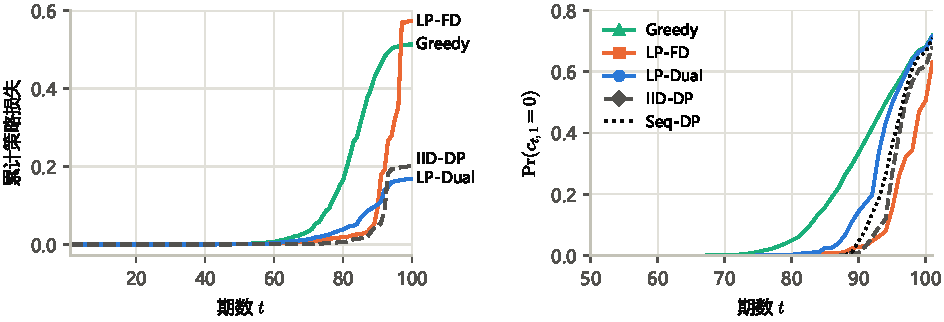
\includegraphics[width=\linewidth]{figures/loss_time.pdf}
\caption{五份数据平均的累计策略损失（左）与商品 1 已售罄的概率 $\Pr(c_{t,1}=0)$（右）}
\label{fig:losstime}
\end{figure}

\subsection{生成序列上的表现}\label{sec:random}
五份给定数据只是众多可能到达顺序中的五个样本。为检验结论是否依赖这五个样本，本文生成了两组序列：500 条人数固定为 $(50,30,20)$ 的随机排列，与给定数据的生成方式相同；500 条按 $\lambda$ 独立同分布生成的序列，各类型人数随机，$F_s$ 介于 \FminIid{} 与 \FmaxIid{} 之间。第\ref{sec:instance}节已说明，五份给定数据可以视为第一组序列的典型样本。表\ref{tab:random}与图\ref{fig:random}给出精确评价的结果。

\begin{table}[htbp]
\centering\small
\caption{生成序列上的精确期望遗憾与策略损失}\label{tab:random}
\begin{tabular}{lrrrrrrrr}
\toprule
 & \multicolumn{4}{c}{随机排列（500 条）} & \multicolumn{4}{c}{独立同分布到达（500 条）} \\
\cmidrule(lr){2-5}\cmidrule(lr){6-9}
策略 & $\overline G$ & $G_{0.95}$ & $G_{\max}$ & $\overline L$ & $\overline G$ & $G_{0.95}$ & $G_{\max}$ & $\overline L$ \\
\midrule
\AlgOne{} & 12.606 & 12.606 & 12.606 & 2.901 & 12.522 & 17.983 & 21.979 & 3.260 \\
\Greedy{} & 10.226 & 10.895 & 11.757 & 0.520 & 9.906 & 16.423 & 18.861 & 0.644 \\
\LPFD{} & 10.200 & 11.099 & 12.927 & 0.495 & 9.711 & 16.331 & 19.674 & 0.449 \\
\LPDual{} & 9.902 & 10.551 & 11.426 & 0.197 & 9.513 & 16.148 & 18.451 & 0.251 \\
\IIDDP{} & 9.801 & 10.421 & 11.044 & 0.096 & 9.370 & 15.987 & 18.207 & 0.108 \\
\bottomrule
\end{tabular}
\par\vspace{0.35em}{\footnotesize $G_{0.95}$ 为 500 条序列上期望遗憾的 95\% 分位数。两组序列的 $F_s$ 与 $V^{\seq}_s$ 逐条计算。}
\end{table}


\begin{figure}[htbp]
\centering
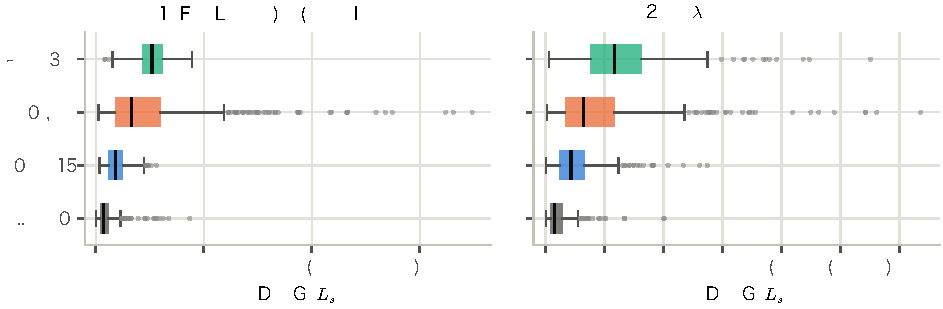
\includegraphics[width=\linewidth]{figures/random.pdf}
\caption{1000 条生成序列上的策略损失分布（箱线图，箱体为四分位区间）}
\label{fig:random}
\end{figure}

随机排列上，\LPDual{} 的平均遗憾为 \GavgDualPerm，低于 \Greedy{} 的 \GavgGreedyPerm{} 与 \LPFD{} 的 \GavgFDPerm{}；它在 \DualBeatsGreedyPerm\% 的序列上不低于 \Greedy{}，在 \DualBeatsFDPerm\% 的序列上不低于 \LPFD{}。\IIDDP{} 的平均策略损失为 \LavgIIDPerm，低于 \LPDual{} 的 \LavgDualPerm，后者在 \DualBeatsIIDPerm\% 的序列上不低于 \IIDDP{}。这一结果符合预期：随机排列接近独立同分布到达，此时 \IIDDP{} 是最优在线策略。\LPDual{} 只需求解规模为 $mn$ 的线性规划，就取得了 \IIDDP{} 的大部分收益。独立同分布序列上的排序相同。

\LPFD{} 的损失分布有一条长尾，最大值为 \LmaxFDPerm，而 \LPDual{} 不超过 \LmaxDualPerm。长尾来自期末的过度预留：\LPFD{} 的策略损失与最后 10 期类型 2 顾客人数的相关系数为 \CorrFDLastTen{}，损失最大的 10 条序列在最后 10 期至多有 \TopFDLastTenMax{} 位类型 2 顾客（期望为 3 位）。\Greedy{} 与 \LPDual{} 的损失则与最后 20 期类型 2 的人数正相关（相关系数分别为 \CorrGreedyLastTwenty{} 与 \CorrDualLastTwenty{}），它们的主要风险是多卖，后段类型 2 顾客越多，越早售罄商品 1 的代价越大。算法 1 的推荐集合只依赖顾客类型，各商品的销量只取决于各类型的人数，与到达顺序无关，因此它在全部 500 条随机排列上的期望收入相同。

\subsection{到达顺序与需求预测}\label{sec:order}
\LPDual{}、\LPFD{} 与 \IIDDP{} 都假设未来顾客按 $\lambda$ 到达。为检验预测失准的后果，本文把三类顾客分块排列，构造六种极端到达顺序，结果见表\ref{tab:order}。

\begin{table}[htbp]
\centering\small
\caption{分块到达顺序下的期望收入}\label{tab:order}
\begin{tabular}{lrrrrrrr}
\toprule
到达顺序 & \Greedy{} & \LPFD{} & \LPDual{} & \LPCount{} & \IIDDP{} & \SeqDP{} & $\E c^{\LPDual}_{T+1,1}$ \\
\midrule
$1\to2\to3$ & 694.050 & 694.200 & 694.199 & 690.984 & 693.735 & 694.543 & 0.851 \\
$1\to3\to2$ & 693.395 & 693.626 & 693.588 & 690.307 & 693.126 & 693.946 & 0.923 \\
$2\to1\to3$ & 696.997 & 674.747 & 683.029 & 696.999 & 670.601 & 697.000 & 2.360 \\
$2\to3\to1$ & 696.806 & 694.261 & 695.511 & 696.782 & 694.757 & 696.812 & 0.830 \\
$3\to1\to2$ & 693.395 & 693.444 & 693.416 & 691.694 & 693.588 & 693.908 & 0.923 \\
$3\to2\to1$ & 696.806 & 696.075 & 696.707 & 696.807 & 696.498 & 696.809 & 0.923 \\
\bottomrule
\end{tabular}
\par\vspace{0.35em}{\footnotesize 表中为精确期望收入，各顺序的 $F_s$ 均为 706。$1\to2\to3$ 表示先到达 50 位类型 1 顾客，再到达 30 位类型 2 与 20 位类型 3 顾客，其余类推。算法 1 在任何顺序下的期望收入都是 \AlgOneER{}。}
\end{table}


顺序 $2\to1\to3$ 下，三种依赖到达率的策略都明显变差：\LPDual{} 为 \BlockDual，\LPFD{} 为 \BlockFD，\IIDDP{} 为 \BlockIID，而 \Greedy{} 达到 \BlockGreedy，与 \SeqDP{} 的 \BlockSeq{} 几乎相同。图\ref{fig:order}显示了原因：第 31--80 期到达的全部是类型 1 顾客，策略仍然预期此后有 30\% 的顾客属于类型 2，按第\ref{sec:behavior}节的预留阈值为它们保留商品 1；实际上第 30 期之后不再有类型 2 顾客，保留的库存最终无人购买。期末商品 1 的期望剩余为 \BlockEconeDual（\LPDual）和 \BlockEconeIID（\IIDDP），\Greedy{} 只剩 \BlockEconeGreedy。损失分解显示，\LPDual{} 的 \LossBlockDual{} 策略损失中，多留占 \HoldBlockDual。\IIDDP{} 对到达率的依赖最强，预留最多，损失也最大。

\LPCount{} 用剩余人数代替到达率预测。顺序 $2\to1\to3$ 下，第 30 期之后它知道不再有类型 2 顾客，商品 1 的对偶价格降为零，于是把商品 1 推荐给类型 1 顾客，期望收入为 \BlockCount，与 \SeqDP{} 相差无几。

但准确的人数信息并不总是有益。顺序 $1\to2\to3$ 下，\LPCount{} 的期望收入只有 \BlockOTTCount，低于 \LPDual{} 的 \BlockOTTDual{} 与 \SeqDP{} 的 \BlockOTTSeq。前 50 期中，\LPCount{} 准确地知道后面还有 30 位类型 2 顾客，按流体模型为他们预留类型 2 对商品 1 的期望需求 12 件。预留量的选择实际上是一个报童问题：类型 2 对商品 1 的需求为 $D_2\sim\mathrm{Bin}(30,0.4)$；多留一件而最终无人购买，损失的是本可卖给类型 1 的净收益 9；少留一件，只是把这件商品卖给了类型 1 而非类型 2，损失为 $10-9=1$。最优预留量是 $D_2$ 的 $1/(1+9)=10\%$ 分位数 \NewsQuantile{} 件。按均值预留 12 件时，期望剩余 \NewsLeft{} 件，期望损失为 \NewsCostMean；按最优预留量，期望损失只有 \NewsCostOpt。\LPCount{} 期末商品 1 的期望剩余为 \BlockOTTEconeCount，\SeqDP{} 为 \BlockOTTEconeSeq。\LPDual{} 第 $t$ 期对后续类型 2 人数的预测是 $0.3(100-t)$ 而非 30，低估了需求，结果少留，反而接近最优。顺序 $1\to3\to2$ 的情况相同（\LPCount{} 为 \BlockOTWCount，\SeqDP{} 为 \BlockOTWSeq）。可见流体模型的问题不只在于预测是否准确：它按期望需求预留库存，忽略了多留与少留之间的代价不对称。

五份给定数据上，\LPCount{} 的平均期望收入为 \ERCount，略低于 \LPDual{} 的 \ERDual。到达顺序接近随机时，按到达率预测已经足够准确；剩余人数信息的价值主要体现在到达顺序有明显结构、且预测偏差会导致多留的场景。

\begin{figure}[htbp]
\centering
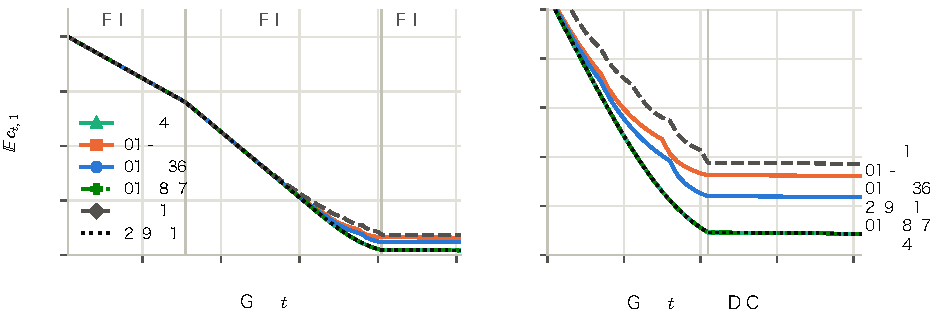
\includegraphics[width=\linewidth]{figures/order_b213.pdf}
\caption{顺序 $2\to1\to3$ 下商品 1 的期望库存 $\E c_{t,1}$。竖线为类型分块的边界，右图为第 60 期之后的局部放大}
\label{fig:order}
\end{figure}

\subsection{库存水平与推荐位数}\label{sec:sens}
把三种商品的库存同比例缩放为 $\lfloor\theta C\rceil$（四舍五入），在五份数据上精确评价各策略，结果见表\ref{tab:theta}与图\ref{fig:theta}。

\begin{table}[htbp]
\centering\footnotesize
\caption{库存缩放 $C\to\lfloor\theta C\rceil$ 下的策略损失（五份数据平均）}\label{tab:theta}
\begin{tabular}{ccrrrrrrrr}
\toprule
$\theta$ & $C$ & $F$ & $\overline{V^{\seq}}$ & $\overline L^{\AlgOne}$ & $\overline L^{\Greedy}$ & $\overline L^{\LPFD}$ & $\overline L^{\LPDual}$ & $\overline L^{\IIDDP}$ & $\overline W^{\AlgOne}$ \\
\midrule
0.3 & $(12,\,11,\,8)$ & 256.0 & 255.996 & 0.173 & 0.006 & 0.006 & 0.006 & 0.000 & 125.81 \\
0.4 & $(16,\,14,\,10)$ & 332.0 & 331.954 & 1.236 & 0.111 & 0.111 & 0.111 & 0.000 & 104.58 \\
0.5 & $(20,\,18,\,13)$ & 422.0 & 421.226 & 7.945 & 1.796 & 1.583 & 1.583 & 0.003 & 80.29 \\
0.6 & $(24,\,21,\,15)$ & 498.0 & 494.473 & 15.256 & 5.685 & 3.174 & 3.174 & 0.067 & 62.04 \\
0.7 & $(28,\,25,\,18)$ & 578.0 & 567.598 & 18.769 & 8.638 & 3.888 & 3.609 & 0.335 & 41.79 \\
0.8 & $(32,\,28,\,20)$ & 629.0 & 618.196 & 12.434 & 4.723 & 1.643 & 1.665 & 0.328 & 26.80 \\
0.9 & $(36,\,32,\,23)$ & 670.0 & 663.494 & 6.250 & 1.521 & 0.738 & 0.457 & 0.289 & 13.99 \\
1.0 & $(40,\,35,\,25)$ & 706.0 & 696.062 & 2.669 & 0.513 & 0.572 & 0.169 & 0.201 & 6.29 \\
1.1 & $(44,\,39,\,28)$ & 724.0 & 715.337 & 0.684 & 0.099 & 0.265 & 0.042 & 0.076 & 1.90 \\
1.2 & $(48,\,42,\,30)$ & 724.0 & 722.424 & 0.107 & 0.012 & 0.064 & 0.006 & 0.016 & 0.35 \\
\bottomrule
\end{tabular}
\end{table}


\begin{figure}[htbp]
\centering
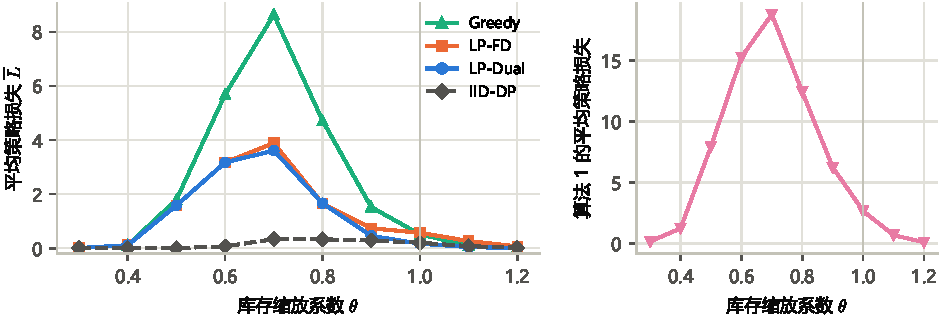
\includegraphics[width=\linewidth]{figures/theta.pdf}
\caption{库存缩放下的平均策略损失（左）与算法 1 的平均策略损失（右）}
\label{fig:theta}
\end{figure}

库存水平决定了在线决策的难度。$\theta\le0.4$ 时三种商品都严重短缺，每件库存几乎都能售出，除算法 1 外各策略都接近最优；$\theta\ge1.1$ 时库存几乎不构成约束，\Greedy{} 已接近最优。中间区域的库存分配最关键：$\theta=0.7$ 时 \Greedy{} 的策略损失达到 \ThetaSevenLGreedy，\LPDual{} 降至 \ThetaSevenLDual，\IIDDP{} 只有 \ThetaSevenLIID。两种 LP 策略在 $\theta\le0.9$ 时表现接近，课程实例 $\theta=1$ 附近的差别来自第\ref{sec:where}节分析的期末过度预留。$\theta=0.6$--$0.8$ 时，LP 策略与 \IIDDP{} 之间仍有约 1.3--3.3 的差距。损失分解显示，$\theta=0.7$ 时 \LPDual{} 的 \LossThetaSevenDual{} 策略损失中有 \SellThetaSevenDual{} 是类型 1 多卖。此时开始的对偶价格为 $\beta=(9,5,0)$，类型 1 顾客对三种商品的评分都是 $0.6$，三者并列，按即时收益推荐了商品 1、2。动态规划的判断不同：库存紧张时商品 1 迟早会售罄，暂不卖给当前的类型 1 顾客几乎没有损失（后来的类型 1 顾客仍会买走它），却保留了卖给类型 2 顾客的机会。流体模型只比较期望值，看不到这种由需求波动产生的期权价值，随机动态规划在库存紧张时因此仍有改进空间。

算法 1 的损失随库存减少而迅速上升。$\theta=0.5$ 时，它平均每条路径推荐 \ThetaHalfW{} 次缺货商品（共 200 个推荐位），策略损失为 \ThetaHalfLAlg；损失在 $\theta=0.7$ 时达到 \ThetaSevenLAlg。这从数量上回答了问题一：库存越紧张，忽略库存造成的损失越大。

\begin{proposition}\label{prop:kn}
当 $K\ge n$ 时，每期推荐全部有货且 $p_{ij}>0$ 的商品在每条样本路径上都达到最大收入
\begin{equation}
R^{*}=\sum_{j=1}^{n}r_j\min\Bigl\{C_j,\ \sum_{t=1}^{T}\ind\{J_t=j\}\Bigr\}.
\end{equation}
\end{proposition}
\begin{proof}
任何策略售出的商品 $j$ 都不超过初始库存，也不超过首选为 $j$ 的顾客人数。推荐全部有货商品时，商品 $j$ 售罄之前每位首选 $j$ 的顾客都会购买，因此销量恰好等于两者中的较小值。
\end{proof}

\begin{table}[htbp]
\centering\small
\caption{推荐位数 $K$ 对期望收入的影响（五份数据平均）}\label{tab:K}
\begin{tabular}{crrrrrrr}
\toprule
$K$ & $F$ & $\overline{V^{\seq}}$ & $\overline{\E R}^{\AlgOne}$ & $\overline{\E R}^{\Greedy}$ & $\overline{\E R}^{\LPFD}$ & $\overline{\E R}^{\LPDual}$ & $\overline{\E R}^{\IIDDP}$ \\
\midrule
1 & 492.0 & 491.992 & 462.772 & 478.001 & 487.070 & 484.848 & 491.992 \\
2 & 706.0 & 696.062 & 693.394 & 695.550 & 695.490 & 695.894 & 695.862 \\
3 & 734.0 & 727.810 & 727.810 & 727.810 & 727.810 & 727.810 & 727.810 \\
\bottomrule
\end{tabular}
\end{table}


表\ref{tab:K}比较了不同推荐位数。$K=3=n$ 时，五种在线策略都推荐全部有货商品（算法 1 推荐全部商品，缺货商品不影响其余商品的成交），期望收入都等于 \KERthreeDual{}，与命题\ref{prop:kn}一致。$K=1$ 时策略之间差异最大：\Greedy{} 为 \KERoneGreedy，\LPDual{} 为 \KERoneDual，\LPFD{} 为 \KERoneFD，\IIDDP{} 达到 \SeqDP{} 的 \KVone。损失几乎全部来自同一类决策：类型 2 顾客对商品 1、2 的即时收益相同（$v_{21}=v_{22}=4$），只有一个推荐位时应当推荐库存充裕的商品 2，把商品 1 留给偏好它的类型 1 顾客。$K=1$ 时类型 1 顾客只看到商品 1，对它的流体需求为 $0.3\tau$。只要 $c_1\ge0.3\tau$，流体模型就认为商品 1 不稀缺，对偶价格为零，类型 2 顾客的两件商品评分并列（均为 4.0），按编号推荐商品 1；$c_1$ 降到 $0.3\tau$ 以下后对偶价格变为正数，才转向商品 2。结果是 \LPDual{} 把商品 1 的库存维持在类型 1 期望需求附近，类型 1 的随机需求超过它时，部分类型 1 顾客买不到商品 1。实际上，向类型 2 推荐商品 2 没有任何代价，\IIDDP{} 从不向类型 2 推荐商品 1。\LPFD{} 的有限差分在库存接近流体需求时先变为正数，较早转向商品 2，损失较小（\LossKoneFD{}，\LPDual{} 为 \LossKoneDual）。这一现象说明，流体模型不重视安全库存：期望需求略低于库存时，它把多余的库存视为零价值。评分并列时以剩余库存作为次级排序依据，是一个可能的改进方向。

\subsection{规模扩展与计算时间}\label{sec:scale}
\textbf{课程实例上的计算时间。} 主实验共 100 万次决策，借助按 $(\tau,c^{\tau})$ 的缓存，\LPDual{} 共求解 \SolvesDual{} 个线性规划，\LPFD{} 求解 \SolvesFD{} 个。不命中缓存的决策中，\LPDual{} 的决策时间中位数为 \TimeDualMedian{} 毫秒，95\% 分位数为 \TimeDualP{} 毫秒；\LPFD{} 分别为 \TimeFDMedian{} 毫秒和 \TimeFDP{} 毫秒。

\textbf{销售期放大。} 把销售期放大为 $T$，库存同比例放大为 $\lfloor TC/100\rceil$，每个 $T$ 生成 10 条人数为 $T\lambda$ 的随机排列并模拟，结果见表\ref{tab:scaling}。\LPDual{} 的遗憾估计在 $T$ 从 25 增至 \ScaleTmax{} 的过程中处于 \ScaleGDualMin--\ScaleGDualMax{} 之间，没有随 $T$ 增长的趋势。$T$ 较大时单条路径收入的标准差随 $\sqrt T$ 增大，遗憾估计的置信半宽随之变宽（$T=\ScaleTmax$ 时为 \ScaleDualHwMax），但 $\overline R^{\LPDual}/F$ 从 $T=25$ 的 95\% 升至 $T=\ScaleTmax$ 的 \ScaleRatioMax\%，相对遗憾持续下降，符合流体近似在大规模下趋于准确的一般结论\cite{gallego,jasin}。\Greedy{} 则不同。在流体近似下，\Greedy{} 以 $0.5\times0.6+0.3\times0.4=0.42$ 的速率消耗商品 1，在 $t^{*}=0.4T/0.42$ 时售罄，此前每期期望收入为 7.24；此后类型 1 改看 $\{2,3\}$，类型 2 只剩商品 2 可买，每期期望收入降为 3.34。商品 2、3 的消耗分别不超过 $0.29T$ 与 $0.13T$，在销售期内不会售罄。于是
\begin{equation}
F-R^{\Greedy}_{\mathrm{fluid}}=7.06\,T-\bigl[7.24\,t^{*}+3.34\,(T-t^{*})\bigr]\approx0.0057\,T,
\label{eq:greedyfluid}
\end{equation}
即 \Greedy{} 的遗憾中有一项随 $T$ 线性增长。单个策略的遗憾估计噪声太大，看不出这一趋势；公共随机数下的配对差则精确得多。表\ref{tab:scaling}中，$T\le100$ 时 \LPDual{} 与 \Greedy{} 的配对收益差不超过 \ScaleGapSmall，此后随 $T$ 近似线性扩大，$T=\ScaleTmax$ 时为 $\ScaleGreedyGapMax\pm\ScaleGreedyGapMaxHw$，与式\eqref{eq:greedyfluid}给出的 \ScaleGreedyFluid{} 量级一致。课程实例的 $T=100$ 规模较小，这一差异被需求波动掩盖；销售期越长、顾客越多，考虑库存机会成本的收益越明显。

\begin{table}[htbp]
\centering\footnotesize
\caption{销售期与库存同比例放大时的遗憾}\label{tab:scaling}
\begin{tabular}{rcrrrrrrr}
\toprule
$T$ & $C$ & $F$ & $\widehat G^{\Greedy}$ & $\widehat G^{\LPFD}$ & $\widehat G^{\LPDual}\pm h$ & $\bar d^{\,\LPDual,\Greedy}\pm h$ & $\overline{F-V^{\seq}}$ & $\overline R^{\LPDual}/F$ \\
\midrule
25 & $(10,9,6)$ & 178 & 8.80 & 9.01 & $8.63\pm0.62$ & $0.17\pm0.09$ & 8.19 & 95.14\% \\
50 & $(20,18,13)$ & 353 & 8.46 & 8.74 & $8.32\pm0.87$ & $0.14\pm0.12$ & 8.60 & 97.64\% \\
100 & $(40,35,25)$ & 706 & 11.30 & 11.34 & $10.94\pm1.02$ & $0.36\pm0.11$ & 9.77 & 98.45\% \\
200 & $(80,70,50)$ & 1412 & 10.22 & 9.73 & $9.66\pm1.81$ & $0.56\pm0.18$ & 9.72 & 99.32\% \\
400 & $(160,140,100)$ & 2824 & 8.86 & 7.56 & $7.50\pm2.67$ & $1.36\pm0.32$ & -- & 99.73\% \\
800 & $(320,280,200)$ & 5648 & 10.26 & 7.29 & $7.57\pm4.61$ & $2.69\pm0.45$ & -- & 99.87\% \\
1600 & $(640,560,400)$ & 11296 & 10.01 & 2.88 & $3.45\pm4.85$ & $6.55\pm0.91$ & -- & 99.97\% \\
\bottomrule
\end{tabular}
\par\vspace{0.35em}{\footnotesize 各 $T$ 独立生成 10 条固定人数的随机排列，人数按 $T\lambda$ 取整后使总和等于 $T$。每条序列模拟 300 次购买（$T=800$ 时 150 次，$T=1600$ 时 100 次），策略共享购买抽样。$\widehat G=F-\overline R$。以每条序列的模拟均值或配对差均值为一个观测，$h$ 是 10 条独立序列间的 95\% $t$ 区间半宽。$T>200$ 时未计算 $V^{\seq}$。}
\end{table}


\textbf{较大的随机实例。} 按 Dirichlet 分布生成购买概率（含不购买选项），价格为 4--20 的整数，到达率也按 Dirichlet 分布生成，库存取算法 1 期望需求的 $\rho$ 倍，$\rho\in\{0.6,0.9\}$，结果见表\ref{tab:large}。这组实验主要检验可行性与计算时间：
\begin{itemize}
\item \textbf{可行性。} 在全部 \LargeInstances{} 个实例、5 种维度组合上，三种库存感知策略都没有推荐缺货商品；算法 1 每条路径平均出现数十到数百次缺货推荐，收入只有离线上界的 \LargeAlgOneMin\%--\LargeAlgOneMax\%，而 \Greedy{} 不低于 \LargeGreedyMin\%。这再次说明问题一中库存过滤的必要性。
\item \textbf{计算时间。} 最大配置的线性规划有 \LargeVars{} 个变量、\LargeRows{} 条约束，处于受限许可证的规模之内。\LPDual{} 的单期决策时间中位数为 \LargeTimeMedian{} 毫秒，95\% 分位数为 \LargeTimeP{} 毫秒；\LPFD{} 每期需要求解至多 $n+1=31$ 个线性规划，中位数为 \LargeTimeFD{} 毫秒。
\item \textbf{收入。} 各配置下 \LPDual{} 相对 \Greedy{} 的平均配对收入差在离线上界的 \LargePairMin\% 与 \LargePairMax\% 之间；逐个实例检验，\LPDual{} 显著较高的有 \LargeSigWins{} 个，显著较低的有 \LargeSigLosses{} 个。这些实例的状态空间过大，无法计算 $V^{\seq}$ 来分解遗憾；从配对差看，库存机会成本带来的改进与课程实例一样较小，且在不同实例上方向不一，不能据此断言 \LPDual{} 在一般实例上优于 \Greedy{}。第\ref{sec:sens}节的灵敏度分析表明，改进的大小取决于库存的紧张程度和顾客偏好的冲突程度。
\end{itemize}

\begin{table}[htbp]
\centering\footnotesize
\caption{随机生成的较大实例}\label{tab:large}
\begin{tabular}{lrrrrrrrrrr}
\toprule
 & & \multicolumn{4}{c}{$\overline R/F$ (\%)} & (\%) & & \multicolumn{3}{c}{单期决策时间/ms} \\
\cmidrule(lr){3-6}\cmidrule(lr){9-11}
$(m,n,T,K)$ & $\rho$ & \AlgOne & \Greedy & \LPFD & \LPDual & $\bar d/F\pm h$ & $\overline W^{\AlgOne}$ & $t^{\LPDual}_{50}$ & $t^{\LPDual}_{95}$ & $t^{\LPFD}_{50}$ \\
\midrule
$(2,5,50,1)$ & 0.6 & 81.9 & 95.6 & 95.4 & 95.9 & $0.29\pm0.17$ & 21 & 0.01 & 0.61 & 0.01 \\
$(2,5,50,1)$ & 0.9 & 90.6 & 96.3 & 96.5 & 96.5 & $0.18\pm0.21$ & 9 & 0.01 & 0.72 & 0.01 \\
$(3,6,100,2)$ & 0.6 & 94.6 & 98.3 & 98.5 & 98.5 & $0.20\pm0.11$ & 81 & 0.52 & 1.14 & 1.04 \\
$(3,6,100,2)$ & 0.9 & 94.0 & 96.7 & 96.6 & 96.7 & $0.00\pm0.14$ & 32 & 0.56 & 1.17 & 1.77 \\
$(5,10,100,3)$ & 0.6 & 92.4 & 97.8 & 97.7 & 97.7 & $-0.07\pm0.06$ & 125 & 0.68 & 1.38 & 2.25 \\
$(5,10,100,3)$ & 0.9 & 89.0 & 92.4 & 92.0 & 92.3 & $0.00\pm0.19$ & 56 & 0.81 & 1.78 & 3.52 \\
$(10,20,200,5)$ & 0.6 & 94.1 & 98.5 & 98.5 & 98.5 & $0.00\pm0.02$ & 424 & 1.33 & 2.66 & 7.02 \\
$(10,20,200,5)$ & 0.9 & 88.4 & 92.4 & 92.1 & 92.4 & $0.00\pm0.15$ & 208 & 1.77 & 3.90 & 11.81 \\
$(20,30,300,4)$ & 0.6 & 90.7 & 98.4 & 98.4 & 98.4 & $-0.02\pm0.06$ & 513 & 2.93 & 5.27 & 22.26 \\
$(20,30,300,4)$ & 0.9 & 84.5 & 91.1 & 91.3 & 91.4 & $0.32\pm0.27$ & 258 & 3.61 & 4.86 & 28.96 \\
\bottomrule
\end{tabular}
\par\vspace{0.35em}{\footnotesize 每种配置随机生成 8 个实例，每个实例 60 次购买重复（$m=20$ 时减半），各策略使用公共随机数。$\rho$ 为库存相对于算法 1 期望需求的比例；$\bar d/F$ 为 \LPDual{} 减 \Greedy{} 的配对收入差占 $F$ 的百分比，$h$ 为 95\% 置信半宽；$\overline W$ 为每条路径上缺货推荐的平均次数；$t_{50}$、$t_{95}$ 为单期决策时间的中位数与 95\% 分位数，包含线性规划求解与排序。}
\end{table}

